%\documentclass[article]{IEEEtran}
%\usepackage[utf8]{inputenc}
%\usepackage{graphicx}
%\usepackage{cite}
%\usepackage{url}

\title{Week 4. GitHub Assignment \\
\large UCCS CS 6000 Computer Science Research}
\author{Jose Luis Castanon Remy}
\date{September 2022}

%\begin{document}

\maketitle

\section{Myself}

During my experience working as a cybersecurity analyst, I have always faced different issues related to the field. I always thought no one had the interest to solve or even address these issues. Common issues that I have found while working are disinformation, disinterest, and uncontrol. This constitutes my second goal. I would love to research and solve issues within the cybersecurity field that no one is paying attention to. One of these issues is the fact that many companies that I had the opportunity to work for, all lack a proper inventory of software leading to security issues.



In addition to my goals and expectations, I consider myself to be very creative. I love to paint. I consider myself an artist in multiple disciplines. I love charcoals and pencils. I am currently learning color theory and how to paint figurines and build dioramas. Apart from my artistic face, I love biking. It is the best way for me to add cardio to my gym routine without getting bored.

I will be completing my Ph.D. in Cybersecurity.


\begin{figure}[htp]
    \centering
    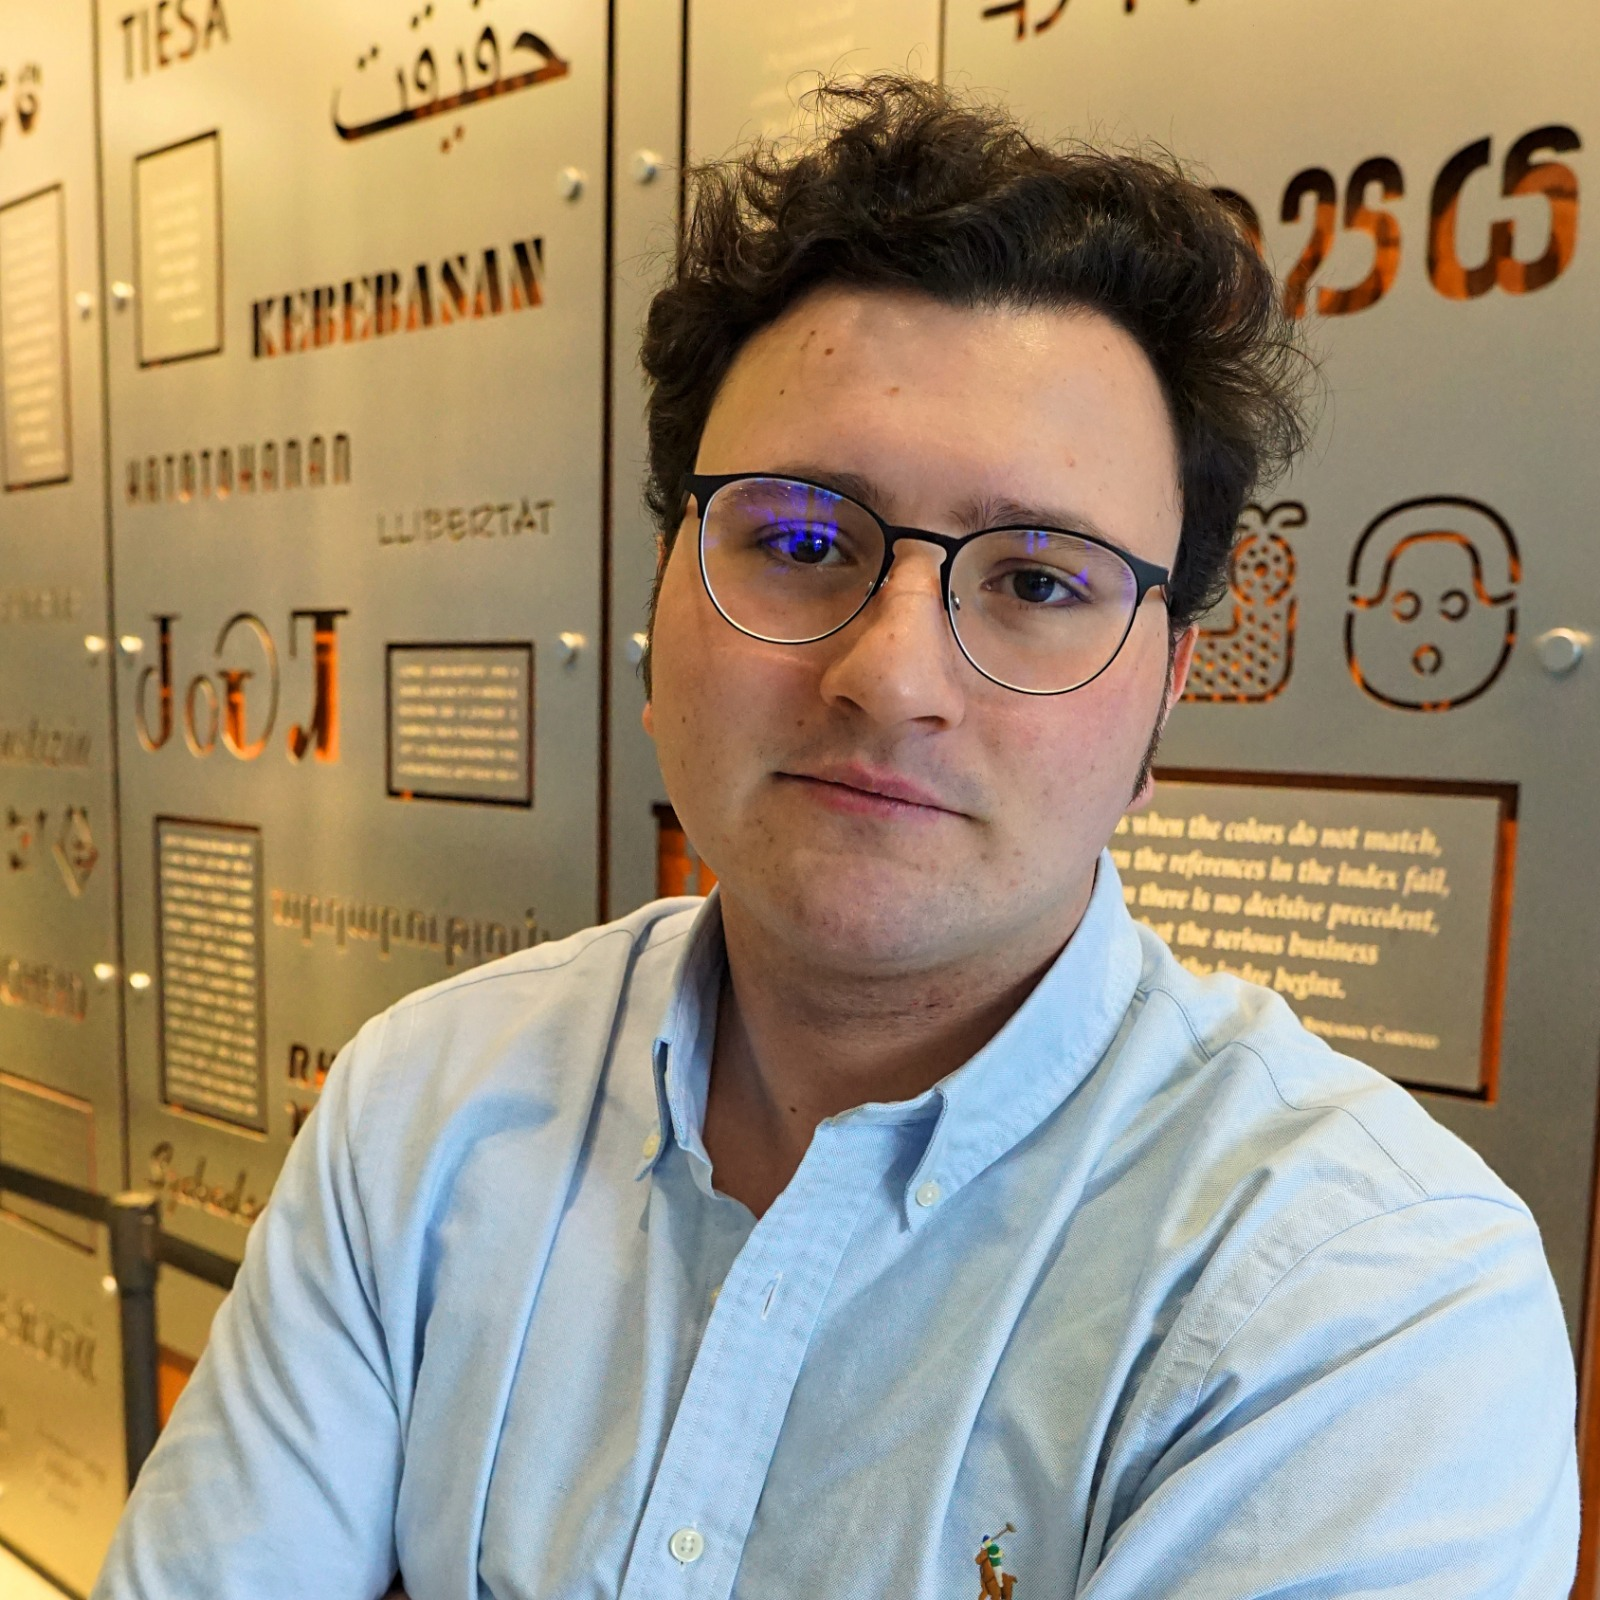
\includegraphics[width=4cm]{UCCSProfileIMG.jpg}
    \caption{An image of myself}
    \label{fig:myself}
\end{figure}


\section{Git Code}
I am currently working on a research related to security and software maintenance. It is a broad topic but I will be trying to narrow it down as I advance with my story.

Maintenance is a large part of every security team. Maintenance represented more than 50\% of the tasks and duties within the last security team I worked with. Part of the maintenance process was related to cleaning. There is a broadly known app related to cleaning called CCleaner. Cleaning helps solve issues directly linked to unused files within installation folders, cache folders, etc. CCleaner helps detect and clean up these files.

Currently, the tasks that CCleaner can perform are limited. For this reason, I have chosen the following Git repo, Winapp2, \url{https://github.com/MoscaDotTo/Winapp2}.

Winapp2 extends the cleaning routines of CCleaner. Winapp2 compiles a list of keys, as a configuration file, for CCleaner to check more applications to clean.
This is highly related to my research as I would like to build something that can map the stack of software within a computer system.
Winapp2 is not also compatible with CCleaner but with other cleaning apps like BleachBit, System Ninja, Avira System Speedup, Tron, and R-Wipe \& Clean. Winapp2 repository contains Winapp2ool, which helps maintain, manage, download and deploy Winapp2, \url{https://github.com/MoscaDotTo/Winapp2/tree/master/winapp2ool}


\section{Questions}
Please, leave your questions after this line.



\bibliographystyle{IEEEtran}
\bibliography{refs}

%\end{document}
